\subsection*{Založení}
\begin{itemize}
	\item Kliknutím na tlačítko vytvoření nových voleb (v záhlaví datagridu) je zobrazen formulář pro editaci voleb.
	\begin{figure}[h]
	\centering
	\includegraphics[width=\linewidth]{tex/attachements/noveVolbyForm.png}
	\captionsetup{width=\linewidth}
	\caption[Formulář založení nových voleb]{Formulář založení nových voleb (zdroj: vlastní)}
\end{figure}
	\item Po vyplnění a odeslání formuláře lze uložené hodnoty upravit pomocí editačního tlačítka na příslušném řádku v datagridu.
	\item Na detail voleb lze přejít kliknutím na tlačítko detailu v příslušném řádku datagridu.
	\begin{figure}[h]
	\centering
	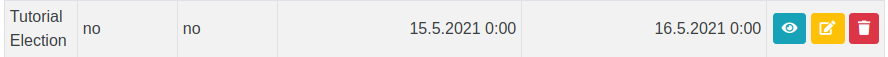
\includegraphics[width=\linewidth]{tex/attachements/noveVolbyGrid.png}
	\captionsetup{width=\linewidth}
	\caption*{Řádek datagridu (zdroj: vlastní)}
\end{figure}
\end{itemize}






\subsection*{Otázky}
Nastavení otázek se provádí na záložce \textit{Questions}. Již přidané otázky jsou zobrazeny v datagridu a lze je upravovat. Nové otázky se přidávají tlačítkem v záhlaví datagridu. Název otázky slouží pro orientaci v seznamu definovaných otázek, voliči není zobrazen. Každá otázka musí mít nastaven minimální a maximální možný počet odpovědí. Limit se při validaci aplikuje pouze pokud je vybrána alespoň jedna odpověď. Pro nepovinné otázky tedy není nutné zadávat limit 0 (aplikace to ani nepovolí). Dalšími poli je text samotné otázky a nastavení zda je odpověď na otázku vyžadována. 

Toto umožňuje dvojí řešení, pokud je vyžadována možnost zdržet se volby (hlasování). Nepovinná otázka umožňuje neodpovídat, ale ve výsledcích voleb není zohledněno, že volič se rozhodl neodpovědět (jinak než porovnáním počtu ostatních možností a odevzdaných hlasů). Druhým řešením je volbu ,,Zdržel se'' zavést jako jednu z možných odpovědí. V takovém případě bude zohleděna tato volba i ve výsledcích. Obdobně by se dalo dívat i na odpověďi ,,Nechci odpovídat'', ,,Nevím'' apod.

V poslední části formuláře je možné přidávat jednotlivé odpovědi. 
\begin{itemize}
\item Další odpovědi lze přidávat kliknutím na tlačítko plus, odebírat tlačítkem minus. 
\item Minimum a maximum možných definic odpovědí je definováno ve zdrojovém kódu formuláře. Výchozí hodnoty jsou minimálně jedna a maximálně pět odpovědí. 
\item Výchozí hodnoty lze přepsat metodami: 
\begin{itemize}
 \item \phpinline{QuestionForm::setMultiplierCopies($copies)} pro minimum a
 \item \phpinline{QuestionForm::setMultiplierMaxCopies($maxCopies)} pro maximum.
\end{itemize}
Tyto metody je ideální volat v místě vytváření formuláře, tedy v \phpinline{ElectionPresenter::createComponentQuestionForm()}. 
\item Změnit výchozí hodnoty napřímo v kódu lze ve třídě \texttt{HasMultiplier}\footnote{\Verb{App\Forms\HasMultiplier}}.

\end{itemize}

Po odeslání formuláře jsou data uložena a otázky i odpovědi je možné upravit opět pomocí editačního tlačítka. Celou otázku lze smazat červeným tlačítkem odpoadkového koše. Jednotlivé odpovědi lze mazat ze samostatné záložky \textit{Answers}.

\subsection*{Seznam voličů}
Seznam voličů vzniká z CSV souboru nahraného prostřednictvím aplikace. 
\begin{itemize}
	\item Aktuální seznam voličů je dostupný přes záložku \textit{Voter List}.
	\item Na záložce \textit{Voter Files} je seznam již nahraných souborů.
	\item Nové soubory lze nahrát prostřednictvím kontextového menu dostupného po kliknutí na ikonu ozubeného kola.
	\item Kterýkoli z nahraných souborů lze aplikovat pro dané volby kliknutím na zelené tlačítko ,,Apply''.
	\item Nahrané soubory lze také smazat nebo stáhnout do počítače a zobrazit jejich obsah.
	\item Smazání nahraného souboru neovlivní již aplikovaný seznam voličů.
\end{itemize}

\subsection*{Spuštění voleb}
Před aktivací voleb je nutné nahrát veřejnou část RSA klíče volební komise prostřednictvím kontextového menu (ozubené kolo). Tento klíč by měl být uložen na bezpečném místě a volební komise by měla zajistit jeho patřičnou zálohu v případě ztráty nebo poškození originálu. Není možné použít klíč chráněný heslem (použitá knihovna \texttt{phpseclib} použití takového klíče nicméně umožňuje a aplikace by k tomu mohla být upravena). Úspěšně nahraný klíč je viditelný na záložce \textit{Overview} v tabulce s šifrovacími klíči.

V tuto chvíli je možné volby aktivovat opět prostřednictvím ozubeného kola.

\subsection*{Ukončení voleb}

\begin{itemize}
	\item Po skončení období nastaveného pro dané volby jsou zpřístupněny další akce na detailu voleb.
	\item Přes kontextové menu je nyní možné nahrát privátní část klíče volební komise.
	\item Po úspěšném nahrání klíče je tento také vidět na záložce \textit{Overview}
	\item Kliknutím na tlačítko ,,Decrypt and count ballots'' na záložce \textit{Results} jsou spočítány odevzdané hlasy
	\item Výsledky voleb jsou zobrazovány i voličům
	\item Pomocí kontextového menu je možné stáhnout volební protokol
	\item Volby je možné deaktivovat přes kontextové menu, neaktivní volby se již nezobrazují voličům.
	\item Ukončené volby včetně všech podstatných náležitostí je možné smazat červeným tlačítkem odpadkového koše v datagridu všech voleb. Veškeré záznamy spojené s těmito volbami budou rovněž odstraněny. Tato akce je nevratná!
\end{itemize}


